%        File: ans_2014_fco.tex
%     Created: June 16, 2014
\documentclass{anstrans}
%%%%%%%%%%%%%%%%%%%%%%%%%%%%%%%%%%%
\title{Extensions to the \Cyclus Ecosystem in Support of Market-Driven 
Transition Capability\\ LLNL-PROC-656426-DRAFT}
\author{Kathryn~D.~Huff$^1$, Massimiliano Fratoni$^1$, Harris R. Greenberg$^2$}

%% uncomment these next five only if using anstrans
\institute{$^1$Department of Nuclear Engineering, University of California, 2150 Shattuck Ave., Suite 230, Berkeley, CA 94709\\
huff@berkeley.edu, maxfratoni@berkeley.edu\\
$^2$ Lawrence Livermore National Laboratory, 7000 East Ave., P.O. Box L-223, Livermore, CA 94551 \\
greenberg6@llnl.gov }
\usepackage{graphicx}
\usepackage{booktabs} % nice rules for tables
\usepackage{microtype} % if using PDF
\newcommand{\units}[1] {\:\text{#1}}%
\newcommand{\SN}{S$_N$}%{S$_\text{N}$}%{$S_N$}%

\usepackage{multicol}
\usepackage{xspace}
\newcommand{\Cyclus}{\textsc{Cyclus}\xspace}

\usepackage{longtable}
\usepackage{placeins}

\setlength{\columnsep}{0.5 in}

\date{}
%%%%%%%%%%%%%%%%%%%%%%%%%%%%%%%%%%%
\begin{document}
%%%%%%%%%%%%%%%%%%%%%%%%%%%%%%%%%%%%%%%%%%%%%%%%%%%%%%%%%%%%%%%%%%%%%%%%%%%%%%%%
\section{Introduction}
% Provide a summary of the work conducted:
%      Describe the technical problem clearly
%      support it with a method

The \Cyclus Fuel Cycle Simulator \cite{carlsen_cyclus_2014} is a framework for 
assessment of nuclear fuel cycle options. This simulation framework is 
incomplete without a suite of dynamically loadable libraries representing the 
process physics of the nuclear fuel cycle (i.e. mining, fuel fabrication, 
chemical processing, transmutation, reprocessing, etc.).  

Within the additional modules repository, Cycamore 
\cite{carlsen_cycamore_2014}, the \Cyclus ecosystem provides some basic 
libraries to represent these processes. However, extension of \Cyclus with new 
capabilities is community-driven, relying on contributions by user-developers.  
This summary describes a set of libraries that have been contibuted to the 
\Cyclus framework to enable market-driven transition analyses. 

\subsection{Motivation}

The attractiveness of a new technology can be assessed to first order by 
evaluating equilibrium fuel cycle scenarios. Equilibrium scenarios are those 
at steady state, in which technologies are deployed statically. However, 
transition dynamics leading up to that equilibrium state also contribute to 
the viability of deploying such a technology.  

For this reason, fuel cycle scenario analysis is often concerned with the 
transition from one reactor technology to another. Such analyses are termed 
``transition scenarios.''  Transition scenarios seek to model the real world 
dynamics of such a technology shift, in part to inform RD\&D decision-making. 

% Why did I do the work?
Transition scenarios are often modeled from a technology availability 
perspective, deploying new technologies based on their readiness.  Arguably, it 
is more realistic to drive a simulation based on market forces (i.e., material 
availability). In that case, technology readiness may be applied only as a 
constraint. 

% What will this work show?
This summary describes additions to the \Cyclus Fuel Cycle Simulator necessary 
to enable market-driven decommissioning and deployment for a specific, 
base-case scenario.  

% What were the central motivations and hypotheses?
% The justification for the objectives.
% Why is the work important?


\subsection{Background}
% Who else has done what?
% How?

Previous fuel cycle simulators have previously achieved market-driven deployment 
capability using look-ahead algorithms for facility deployment 
\cite{schneider_nfcsim:_2005}.  These simulators typically conduct guess-and-check 
simulation attempts, restarting or crashing if their algorithm failed to 
generate a coherent simulation.

% What has this group previously done?

The development version of the \Cyclus simulator has long been capable of 
technology driven scenarios \cite{gidden_once_2012}, those scenarios relied 
on explicit demand or deployment profiles defined by the user. This capability 
shares the disadvantages of the guess-and-check methods of other simulators, 
since the user-defined deployment profiles may lead to incongruous scenarios 
(i.e., insufficient material or processing availability and unexpected idle 
facilities).  

However, the \Cyclus simulator, due to its dynamic resource exchange paradigm, 
is capable of dynamically checking material availability in the simulation and 
responding accordingly.  

% Guidance to the reader

By harnessing the \Cyclus resource exchange paradigm, and emphasizing 
generality, the Agents contributed in this work enable market-driven transition 
scenarios for a range of future use cases in the \Cyclus ecosystem. 

% What should the reader watch for in the paper?
% What are the interesting high points?
% What strategy did we use?

\subsection{Method}
% Summary/Conclusion
% What should the reader expect as conclusion?
% What does it mean?
% What hypotheses do I mean to  test?
% What did I actually test?

Extensions to the \Cyclus framework are necessary because the available
institution, region, and facility archetypes packaged with the Cycamore
repository are not sufficient to model the specific goals of all simulation 
descriptions.  In this case, Facility Agents were contributed to support 
reprocessing and fuel fabrication specifications in the transition scenario
definition of interest and an Institution Agent was contributed to support 
market-driven decommissioning of old technologies.  


This is a canonical example of a user-developer's workflow for capability 
extension in \Cyclus. That is, each scenario specification of interest in fuel
cycle analysis is usually sufficiently pathological that modifications must
almost always be made in any simulation framework. This effort demonstrates how 
the modularity built into
the \Cyclus framework allows extension without modification of the core logic.  

 

%%%%%%%%%%%%%%%%%%%%%%%%%%%%%%%%%%%%%%%%%%%%%%%%%%%%%%%%%%%%%%%%%%%%%%%%%%%%%%%%
\section{Simulation Description}
\subsection{Scenario Definition}
The simplified transition scenario modeled was from the current once-through
Light Water Reactor (LWR) fuel cycle, to a fleet of Sodium Fast Reactors (SFR)
with 100\% recycle of spent fuel.  The simulation starts in January 2014 and
lasts until transition to 100\% SFRs is complete. The nuclear installed
capacity is constant (100GWe).

The transition is driven by the criteria that when sufficient separated
material is present, an LWR ($1000$MWe) should be decommissioned and replaced
with three ($333.\bar{3}$) SFRs.

A summary of the material flows in the simulation can be found in Figure 
\ref{fig:cycic_img}. 

\begin{figure}[htpb!]
\begin{center}
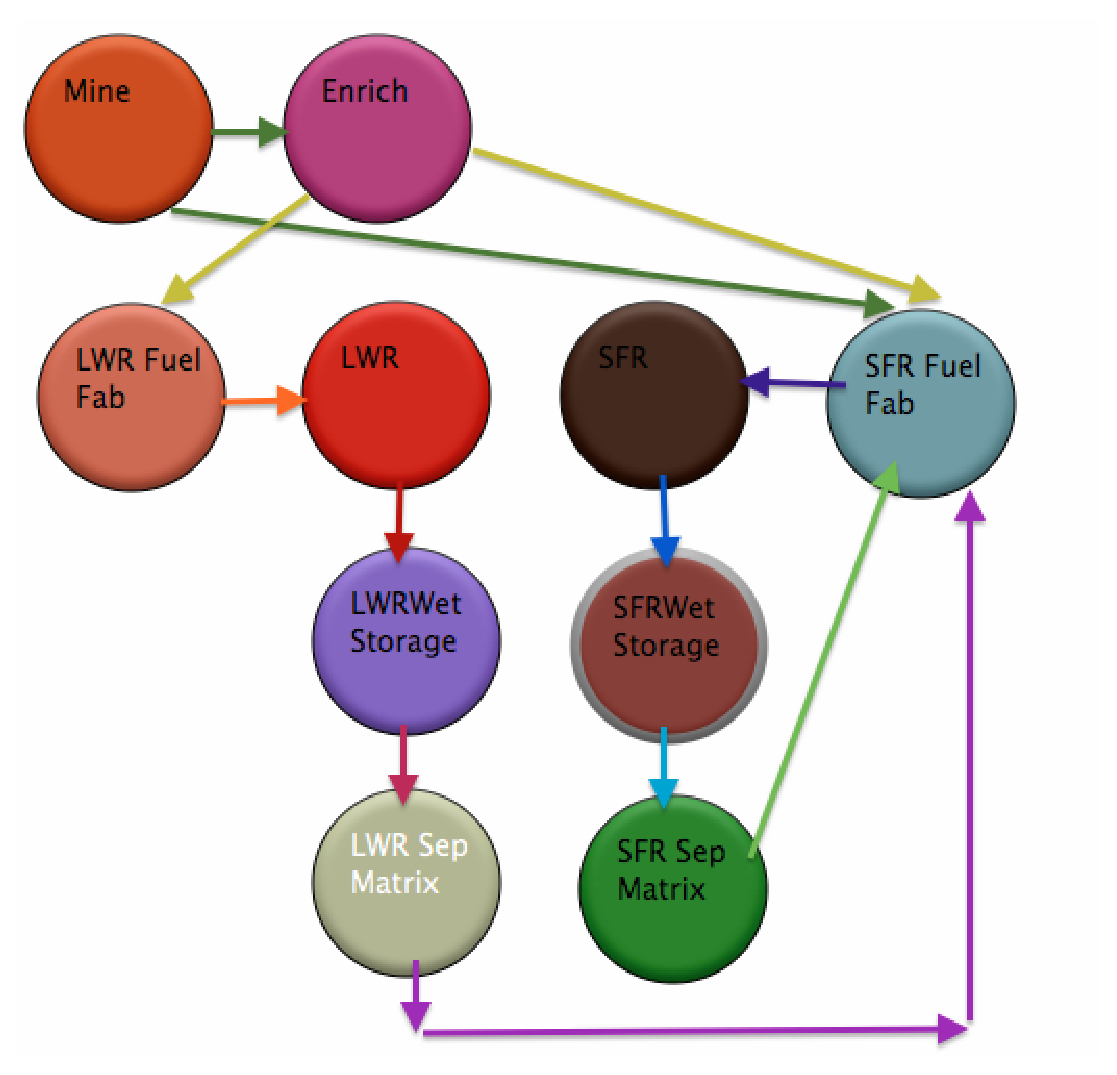
\includegraphics[width=0.45\textwidth]{cycic_img.eps}
\end{center}
\caption{The basic material flow paths for this simulation. This image was 
generated by Cycic, the input controller for \Cyclus 
\cite{flanagan_input_2013}.}
\label{fig:cycic_img}
\end{figure}

\subsubsection{Deployment Regions and Institutions}

In order to facilitate a deployment profile for the LWR to SFR transition, an 
existing Cycamore model was used. The GrowthRegion model maintains a 
power generation profile specified by the user. It does this by deploying or 
decommissioning reactors when necessary to maintain the specified growth 
profile.  

In this case, a constant 100GWe ``growth'' is maintained in the simulation. 
This region encapsulates all of the facilities in this simulation. 
When sufficient material is available to support a new set of three SFRs, an 
LWR is decommissioned. When power generating capacity is lost due to an LWR 
(1000MWe) decommissioning, the GrowthRegion deploys sufficient SFR capacity 
(three 333.3MWe SFRs) to replace it. 

An entity that decommissions LWRs based on material availability was not 
present in the default models, however. To support this ability, an extension 
model was implemented as a ``Decommissioning Facility.'' That model is 
addressed in Section \ref{sec:decomminst}.

\subsubsection{Commodities}

%\begin{multicols}{1}
\begin{table}[htbp!]
\centering
\begin{tabular}{|l|l|l|}
\hline
Commodity  &     Offered By  &    Requested By \\
\hline
Natural  U & Mine & Enrichment \\ 
LEU & Enrichment & LWRFuelFab \\ 
Depleted U & Enrichment & SFRFuelFab \\ 
fresh LWR fuel & LWRFuelFab & LWR \\ 
fresh SFR fuel & SFRFuelFab & SFR \\ 
LWR UNF & LWR & LWRWetStorage \\ 
SFR UNF & SFR & SFRWetStorage \\ 
cool LWR UNF & LWRWetStorage & LWRSeparation \\ 
cool SFR UNF & SFRWetStorage & SFRSeparation \\ 
separated LWR U & LWRSeparation & SFRFuelFab \\ 
separated LWR TRU & LWRSeparation & SFRFuelFab \\ 
separated SFR U & SFRSeparation & SFRFuelFab \\ 
separated SFR TRU & SFRSeparation & SFRFuelFab \\ 
\hline
\end{tabular}
\caption{Commodity flow in the transition simulation}
\label{tab:commods}
\end{table}
%\end{multicols}
Note that the exact compositions of U and TRU were not given. These will be
approximated by representative isotopes in the \Cyclus definition.

\subsubsection{Facility Implementations}

\begin{table}[htbp!]
\centering
\begin{tabular}{|l|l|r|}
\hline
\textbf{Facility Type} &\textbf{Agent} & \textbf{Key Parameters}\\
\hline
Mine & SourceFacility & Capacity\\
\hline
Enrichment & EnrichmentFacility & feed enrchment\% \\
& & tails enrichment\% \\
& & Process time \\
\hline
LWRFuelFab & StreamBlender & Process time\\
& & Fissile Source\\
\hline
SFRFuelFab & StreamBlender  & Process time\\
& & Fissile Sources\\
& & Fertile Sources\\
\hline
LWR & BatchReactor & Installed Capacity \\
& & Capacity Factor \\
& & Batches per core \\ 
& & Cycle length\\
& & Fresh Fuel Comp. \\
& & Spent Fuel Comp. \\
\hline
SFR & BatchReactor & Installed Capacity\\
& & Capacity Factor \\
& & Batches per core \\ 
& & Cycle length\\
& & Fresh Fuel Comp. \\
& & Spent Fuel Comp. \\
\hline
LWRWetStorage & CommodConverter & Process time\\
\hline
SFRWetStorage & CommodConverter & Process time\\
\hline
LWRSeparation & SeparationMatrix & Capacity\\
& & Process Time\\
& & Efficiency Matrix\\
\hline
SFRSeparation & SeparationMatrix & Capacity\\
& & Process Time\\
& & Efficiency Matrix\\
\hline
HLW Repository & SinkFacility & Capacity \\
\hline
\end{tabular}
\caption{Facilities and their implementations with key parameters.}
\label{tab:facimpl}
\end{table}
\FloatBarrier

\subsubsection{Desired Outputs}

The desired outputs of this simulation include deployment metrics such as the 
year during which the transition becomes complete and capacity profiles over 
time. These profiles should demonstrate that there were no potential generating 
shortages. Additionally, material metrics such as separated surplus PU or TRU 
profiles, LWR used fuel reprocessing rate (t/yr), SFR used fuel reprocessing 
rate (t/yr),  LWR used fuel mass in storage (t), and SFR used fuel mass in 
storage (t).

\input{existingfacs}

%%%%%%%%%%%%%%%%%%%%%%%%%%%%%%%%%%%%%%%%%%%%%%%%%%%%%%%%%%%%%%%%%%%%%%%%%%%%%%%%
\section{Capability Extensions}

% --------------------------------------------------------------
\begin{frame}[fragile]
  \frametitle{Storage Facility}
Two storage facilities were needed. One would conduct spent fuel cooling from
the LWRs and the other would do the same for the SFRs. 
\begin{figure}[htbp!]
\begin{center}
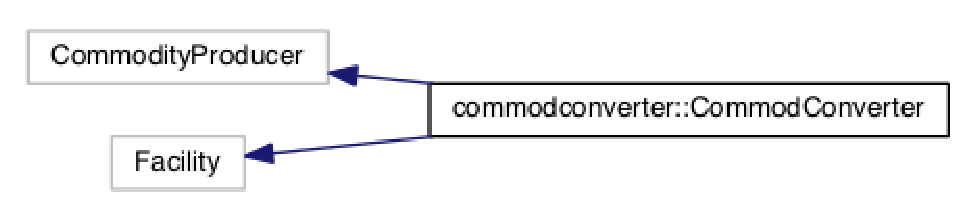
\includegraphics[width=0.8\textwidth]{cc_inherit}
\end{center}
\caption{Utilizes interfaces defined in Cyclus.}
\label{fig:cc_inherit}
\end{figure}
\end{frame}
% --------------------------------------------------------------
\begin{frame}[fragile]
  \frametitle{Storage Archetype Definition}
Only one archetype is needed for this:  a simple representation of timed commodity transformation. 
 I called it CommodityConverter 
 (\url{https://katyhuff.github.io/CommodConverter}) \cite{huff_market_2014}, and it accepts the following configuration variables:
\begin{itemize}
\item incoming commodity
\item outgoing commodity 
\item maximum capacity
\item delay time
\end{itemize}
\end{frame}
% --------------------------------------------------------------
\begin{frame}[fragile]
  \frametitle{Storage Behavior}
After receiving a resource
(e.g., a material), this facility waits for a user-defined time period. Once
that time period has passed, the resource is offered to the resource exchange
system as a new commodity type. 
\end{frame}
% --------------------------------------------------------------
\begin{frame}[fragile]
  \frametitle{Code To Code Input Snippet}
\begin{lstlisting}
  <facility>
    <name>LWRWetStorage</name>
    <lifetime>1200</lifetime>
    <config>
      <CommodConverter>
        <in_commod>lwr_unf</in_commod>
        <in_recipe>lwr_unf_recipe</in_recipe>
        <out_commod>lwr_unf_cool</out_commod>
        <out_recipe>lwr_unf_recipe</out_recipe>
        <process_time>48</process_time>
      </CommodConverter>
    </config>
  </facility>
\end{lstlisting}
\end{frame}

\subsection{Stream Blender Facility : Fuel Fabrication}

The process of fuel fabrication from separated materials streams can most
concisely be described as blending into a recipe. To most generically represent
this process, the Stream Blender Facility has been added to the \Cyclus 
ecosystem.  This new Facility Agent handles the combination of various 
commodity streams in appropriate proportions to acheive a goal recipe.  

\begin{table}[h!]
\centering
\begin{tabular}{|l|r|r|r|}
\hline
\textbf{Parameter} & \textbf{Units} & \textbf{Default} & \textbf{Range}\\
\hline
Input Commodities & set of strings& ``''& \\
Output Commodities & set of strings&``'' & \\
Waste Commodity & string & ``waste'' & \\
Production Capacity& kg/month& $\infty$& $0-\infty$\\
Process Time& months & $0$ & $0-\infty$ \\
Source Preferences& - & - & - \\
Goal Recipe& mass vector & - & -  \\
\hline
\end{tabular}
\caption{Input parameters for the Stream Blender Facility Agent}
\label{tab:commodconverter}
\end{table}

\subsection{Matrix-Based Separation Facility Model}

By describing the separations process as a simple matrix of efficiencies, a  
material stream transformation can be conducted. The specific process chemistry 
for the separation at hand is treated as elemental, as representative of a 
  non-laser separations process. The efficiencies must be defined to transform 
  an incoming composition vector $I$ with $N$ constituent amounts, $I_n$ to an 
  outgoing set of $M$ streams, $E_m$. The efficiency matrix $\eta$ is therefore 
  an $N\times M$ matrix of efficiencies. The matrix of separation efficiencies 
  has a default value: the identity matrix of size $N\times N$. In this 
  context, the identity matrix represents complete and perfect elemental 
  separation without losses. 

\begin{align}
  \left[
    \begin{array}{c c c c c c c}
      \eta_{11} & . & . & . & . & . & \eta_{1M} \\
      \eta_{21} & . & . & . & . & . & \eta_{2M} \\
      . & . & . & . & . & . & . \\
      . & . & . & . & . & . & . \\
      . & . & . & . & . & . & . \\
      \eta_{N1} & .  & . & . & . & . & \eta_{NM} \\
    \end{array}
    \right]
  \left[
    \begin{array}{c}
      I_1\\
      I_2\\
      . \\
      . \\
      . \\
      I_N\\
    \end{array}
    \right]
    =
    \left[
      \begin{array}{ c }
        E_1\\
        E_2\\
        .\\
        .\\
        .\\
        E_M\\
      \end{array}
      \right]
\label{defaultsep}
\end{align}

For realistic separations, the user is expected to produce an efficiency 
matrix representing the separations technology of interest to them. 
By requesting the feedstock from the 
appropriate markets, the facility acquires an unseparated feedstock stream. 
Based on the input parameters  in Table \ref{tab:sepmatrix}, the separations 
process proceeds within the timesteps and other constraints of the simulation. 

\begin{table}[h!]
\centering
\begin{tabular}{|l|r|r|r|}
\hline
\textbf{Parameter} & \textbf{Units} & \textbf{Default} & \textbf{Range}\\ 
\hline
In-Commodity & string &``'' & any string \\
$\eta$ Matrix & \% yield & Identity & positive matrix \\
\hline
\end{tabular}
\caption{Input parameters for the Matrix-Based Separation Facility Model}
\label{tab:sepmatrix}
\end{table}

Thereafter, separated streams as well as a stream of losses are offered the 
appropriate markets for consumption by other facilities. In the transition 
scenario at hand, the StreamBlender fuel fabrication facility purchases the 
streams it desires in order to produce SFR fuel. 

\begin{frame}[fragile]
\frametitle{Market-Driven Institution}
Needed : An institution that can peek into the Resource Exchange and decommission LWRs when enough SFR fuel is available.
\begin{figure}[htbp!]
\begin{center}
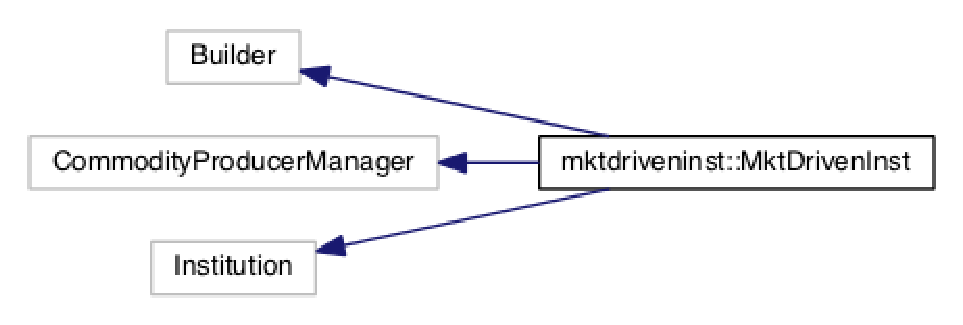
\includegraphics[width=0.8\textwidth]{mdi_inherit}
\end{center}
\caption{Utilizes interfaces defined in Cyclus.}
\label{fig:mdi_inherit}
\end{figure}
\end{frame}

\begin{frame}[fragile]
\frametitle{Market-Driven Institution}
This institution is undergoing further testing, but will enable a large range 
of transition-focused simulation scenarios
(\url{https://katyhuff.githug.io/MktDrivenInst})\cite{huff_market_2014}.
\end{frame}


%%%%%%%%%%%%%%%%%%%%%%%%%%%%%%%%%%%%%%%%%%%%%%%%%%%%%%%%%%%%%%%%%%%%%%%%%%%%%%%%
\section{Results and Analysis}
% Provide your results:
%       clearly

To extend the capabilities of the \Cyclus ecosystem to include market-driven 
building and decommissioning, physics agnostic separations, simple storage, and 
source-preferential fuel fabrication, the following Agents were developed:

\begin{itemize}
\item SeparationsMatrix Facility, physics agnostic separations, (https://github.com/katyhuff/separationmatrix)
\item CommodConverter Facility, timed-release storage, (https://github.com/katyhuff/commodconverter)
\item StreamBlender Facility, source-preferential fuel fabrication, (https://github.com/katyhuff/streamblender)
\item MktDrivenInst, a market-driven institution, (https://github.com/katyhuff/mktdriveninst)
\end{itemize}



\section{Acknowledgements}

This work was conducted <LLNL text>.

Additionally, this material is based upon work supported by the Department of 
Energy National Nuclear Security Administration under Award Number(s) 
DE-NA0000979. % Katy's appointment is NSSC, must acknowledge for everything

<disclaimer text>.



%%%%%%%%%%%%%%%%%%%%%%%%%%%%%%%%%%%%%%%%%%%%%%%%%%%%%%%%%%%%%%%%%%%%%%%%%%%%%%%%
\bibliographystyle{ans}
\bibliography{bibliography}
\end{document}


